\section{Actuator Construction and Multibody Interface}
\label{sec:construction}
\subsection{Subsystem Boundary and Repeated Structure}
Each of the four hydraulic axes is built as an \textnormal{Actuator\_i} subsystem. The boundary contains one Simulink command input, two multibody frame connections, and two isothermal-liquid connections named P and T. Inside this boundary are the directional valve, double-acting actuator, an external translational friction element, barrel and rod CAD bodies, alignment joints, the prismatic actuation joint, pressure taps, and force/extension sensing. This organization makes the hydraulic drive and its mechanical installation one reusable unit rather than an ideal torque applied to an arm joint.

Table~\ref{tab:branches} relates the actuator names to the imported mechanical parts. The fifth command follows a different implementation: \textnormal{Actuator\_5} is a Simulink--PS conversion feeding the cutting-head revolute joint's torque input. It contains no pump connection, valve, or double-acting cylinder. Accordingly, the integrated model has five command channels but four hydraulic actuator branches.

\begin{table*}[t]
\caption{Actuation Branches and Mechanical Installation in the Saved Model}
\label{tab:branches}
\centering\small
\begin{tabular}{llll}
\hline
Command & Subsystem & Imported cylinder/mechanism & Mechanical role\\\hline
$u_1$ & Actuator\_1 & Ausleger\_Schwenkzylinder & Base-to-swing installation\\
$u_2$ & Actuator\_2 & Hebezylinder & Swing assembly to first boom\\
$u_3$ & Actuator\_3 & Knickzylinder & First boom to second boom\\
$u_4$ & Actuator\_4 & Messerkopf\_Schwenkzylinder & Second boom to cutting-head swivel linkage\\
$u_5$ & Actuator\_5 & Messerkopf\_link\_joint & Direct physical-signal torque command\\\hline
\end{tabular}
\end{table*}

\begin{figure*}[t]
\centering
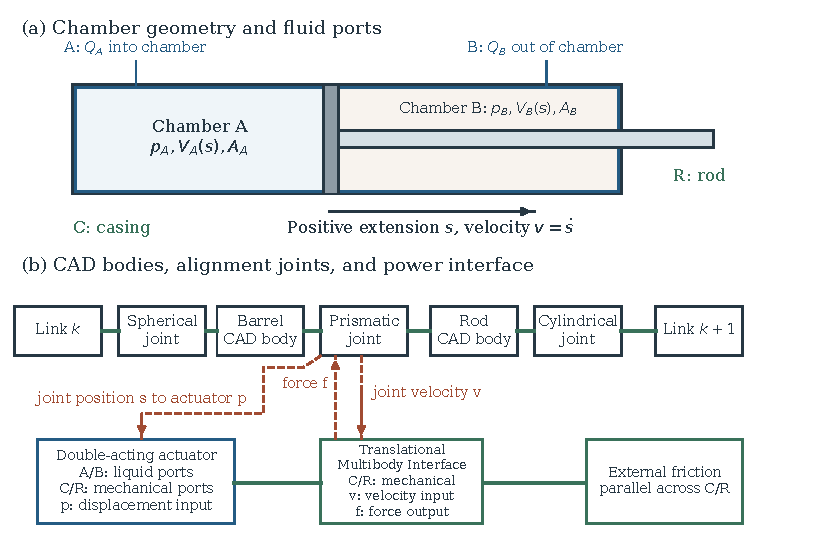
\includegraphics[width=.94\textwidth]{figures/cylinder-construction.pdf}
\caption{Actuator construction. (a) Symbolic chamber geometry, fluid ports A/B, casing C, rod R, and positive extension. Chamber areas are symbolic; the saved active blocks use equal A/B areas as listed in Table~\ref{tab:cylinders}. (b) CAD barrel and rod bodies form a closed chain between adjacent arm links through spherical, prismatic, and cylindrical joints. The prismatic joint supplies position and velocity; the translational interface returns axial force. Solid green connections represent mechanical coupling and dashed red connections represent physical signals. The friction element acts in parallel across the actuator's translational terminals.}
\label{fig:construction}
\end{figure*}

\subsection{Building the Mechanical Cylinder Assembly}
The barrel (\textnormal{Rohr}) and rod (\textnormal{Kolben}) remain separate solid bodies so that their imported mass, inertia, and attachment frames participate in the multibody equations. Rigid transforms place joint frames on the CAD attachment axes; the visible mesh alone does not define the cylinder axis. The spherical connection attaches the barrel assembly to the upstream link and permits alignment. The internal prismatic joint permits rod translation along the cylinder axis. The rod-side cylindrical connection provides angular alignment while its axial coordinate is constrained by very tight stored limits. It is therefore not intended to introduce a second freely extending stroke.

The main arm retains its revolute joints. The cylinder forms a second mechanical path between two arm links, so changing cylinder extension changes the revolute configuration through loop closure. An imposed joint-angle trajectory and a force-driven cylinder must not independently prescribe incompatible motion to the same closed loop.

The construction sequence is to import the arm and attachment frames, insert the separate barrel/rod bodies, align the prismatic axis, connect the spherical and cylindrical ends, and check assembly in the initial configuration. Next, enable prismatic position/velocity sensing and force input, then connect the hydraulic interface. Finally, check the sign of a small commanded extension against the resulting joint motion. This sequence separates frame-assembly problems from hydraulic initialization and controller tuning.

\subsection{Connecting Hydraulic Power to the Prismatic Joint}
The Double-Acting Actuator (IL) has liquid ports A/B and translational conserving ports C/R. C represents the casing and R the rod. In the saved model, C is connected to the translational reference and to the interface casing terminal; R is shared by the actuator, external friction element, and interface rod terminal. This reference fixes the scalar translational coordinate system. It does not ground the moving barrel CAD body in the three-dimensional arm.

The Translational Multibody Interface receives the prismatic joint's sensed relative velocity at its physical-signal input v and supplies the force signal f to that joint's force-actuation port~\cite{interface}. The joint's sensed position is also connected directly to the actuator's p input and to the extension sensor. The actuator is configured to receive displacement from the multibody joint, rather than independently integrating a second position state~\cite{actuator}. Thus the position-dependent chamber volume uses the same motion that produces translational velocity.

For an ideal interface the transmitted quantities satisfy
\begin{equation}
P_{\mathrm{trans}}=F_{\mathrm{int}}v_c,
\qquad v_c=\dot{s}_{\mathrm{joint}}.
\end{equation}
The frame ordering, mechanical orientation, and signal signs must be consistent with this relation. Reversing a sensed velocity without reversing the corresponding force convention changes the apparent power transfer. The force log denotes the interface signal, not an independently measured external load.

\subsection{Cylinder Geometry, Initial State, and Stroke Limits}
Positive extension increases chamber A volume and decreases chamber B volume. Dead volumes keep the pressure states finite near a stroke end. For a conventional single-rod cylinder, geometric areas can be obtained from bore diameter $d_b$ and rod diameter $d_r$ as
\begin{equation}
A_A=\frac{\pi d_b^2}{4},\qquad
A_B=\frac{\pi(d_b^2-d_r^2)}{4}.
\end{equation}
However, these geometric relations must not be used to silently replace the actual saved block values. The active cylinders in this model use equal A/B effective areas. The general asymmetric-cylinder equations remain useful, but the stored configuration is an equal-area parameterization rather than evidence of an identified single-rod bore.

\begin{table*}[t]
\caption{Literal Active Cylinder and External Friction Settings}
\label{tab:cylinders}
\centering\small
\begin{tabular}{lrrrrrr}
\hline
Branch & $A_A=A_B$ (m$^2$) & Stroke (m) & $V_{A0}=V_{B0}$ (m$^3$) & Stored $p_{A0}$ (MPa) & Stored $p_{B0}$ (MPa) & $b_v$ (N\,s/m)\\\hline
1 & 0.2513274 & 1.85 & $10^{-4}$ & 3.548700 & 24.232950 & $10^8$\\
2 & 0.2513274 & 1.85 & $10^{-4}$ & 3.548700 & 24.232950 & $10^8$\\
3 & 0.1256600 & 2.25 & $10^{-4}$ & 7.685550 & 13.890825 & $10^7$\\
4 & 0.1256600 & 2.25 & $10^{-4}$ & 7.685550 & 13.890825 & $10^7$\\\hline
\end{tabular}
\end{table*}

Table~\ref{tab:cylinders} records values and units read directly from the active blocks; the pressure entries are stored initialization parameters and are not measured operating pressures or guaranteed enforced initial conditions. The piston offset is the expression \textnormal{(hydr\_x0)-hydr\_stroke}. Its evaluated value and initialization priority must be checked with the model workspace. The external friction blocks have breakaway/Coulomb forces of 200,000/200,000~N on branches 1/2, 1,000/1,000~N on branch 3, and 2,000/2,000~N on branch 4; the stored breakaway speed is 0.060623~m/s. These large effective areas and friction settings should be reconciled with geometry and units before a new physical-accuracy claim is made.

Dynamic chamber compressibility is enabled in all four active actuator blocks. Their built-in cylinder-friction, internal-leakage, and end-cushion options are disabled; friction is instead represented by the separate parallel element. The prismatic joints on branches 2--4 also store 5,000~N\,s/m damping, while branch 1 stores zero. This damping is an additional mechanical contribution and must not be confused with the external friction coefficient.

The prismatic lower/upper limit flags are enabled only on branch 2, at $-0.2$ and $0.2$~m. Branches 1, 3, and 4 retain numerical limit fields with their activation flags off. The actuator's own stroke/hard-stop settings and the cylindrical alignment-joint limits remain separate constraints. Stored bound fields alone do not activate a joint limit.

\begin{figure*}[t]
\centering
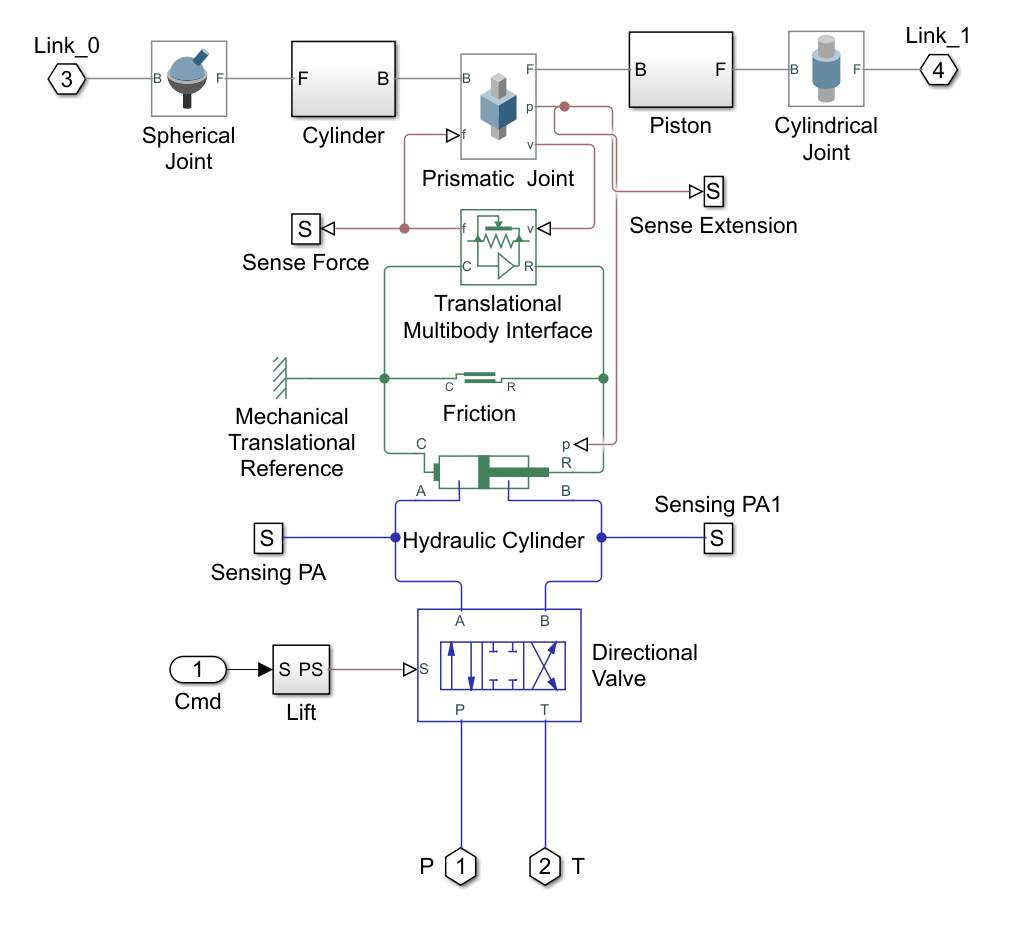
\includegraphics[width=.63\textwidth]{figures/actuator-subsystem-original.png}
\caption{Original project view of a complete electro-hydraulic actuator subsystem. Command conversion drives valve S; P/T join the common rails, and A/B join the sensed cylinder chambers. The middle network contains the translational actuator, parallel friction, reference, and interface. The upper closed chain contains the barrel, force-actuated prismatic joint, rod, and alignment joints. The physical-signal connections return position/velocity and apply force. The image records the project construction rather than a new run.}
\label{fig:actuator-original}
\end{figure*}

\section{Hydraulic Network and Signal Integration}
\subsection{Complete Circuit Organization}
The documented circuit is a shared supply/return arrangement with a fixed-displacement pump, reservoir, pressure-relief path, fluid-properties definition, pressure/flow sensing, and four parallel actuator modules. The pump converts imposed shaft rotation to fluid flow. Each valve meters this common flow into one cylinder chamber while allowing fluid from the other chamber to return. A relief path limits pressure only when its orientation, setpoint, and connection to the pressure rail are correct. The accumulator is part of the documented design, but its block is commented out in the saved editable model.

\begin{figure*}[t]
\centering
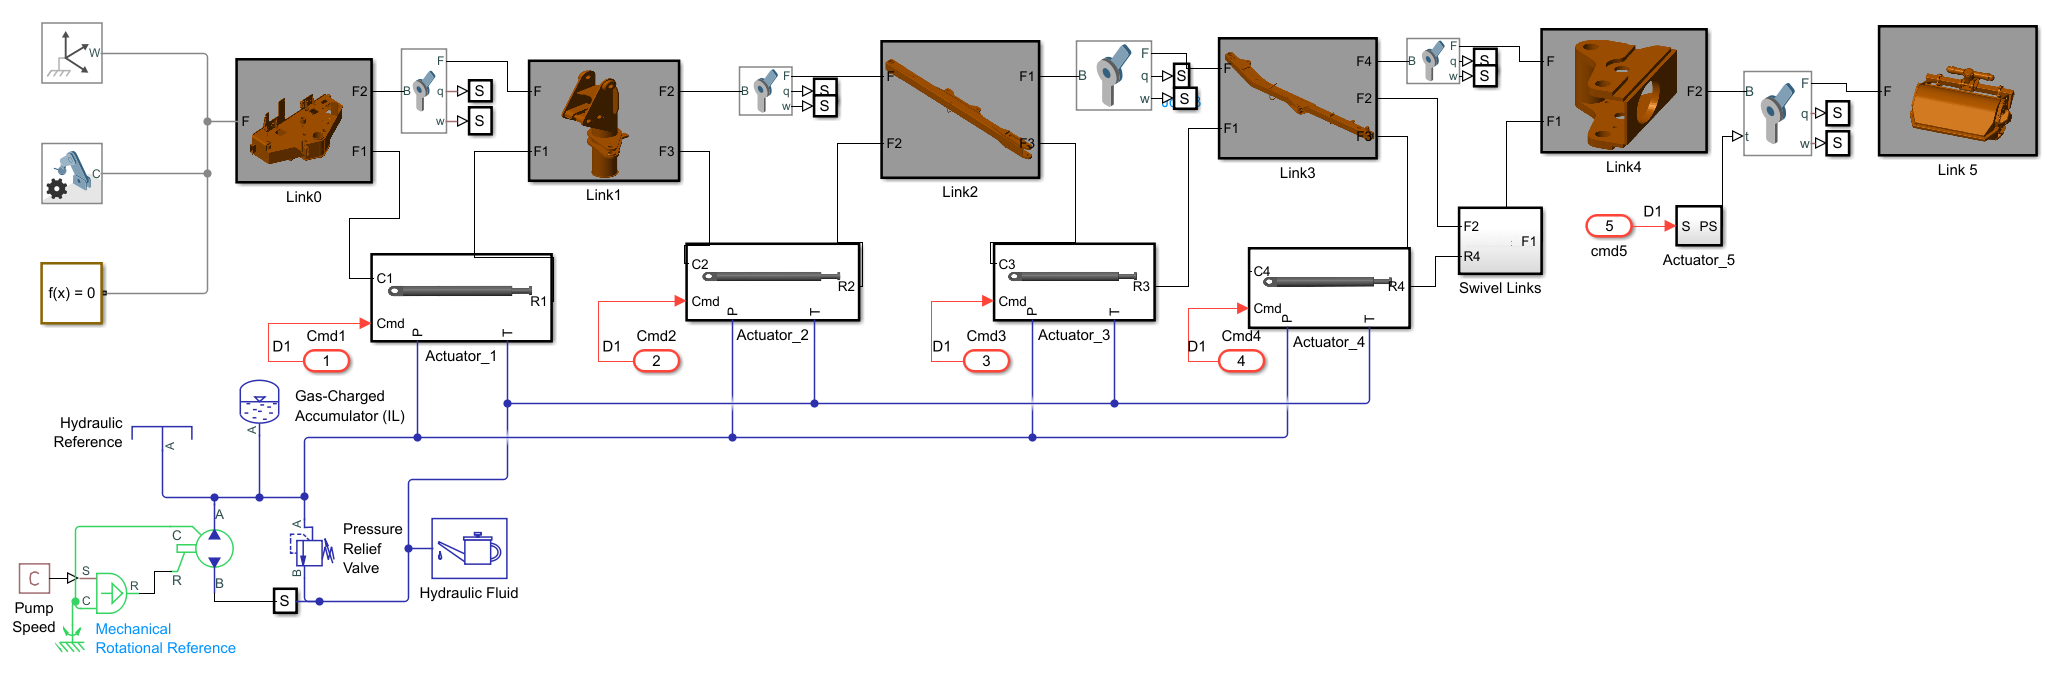
\includegraphics[width=\textwidth]{figures/integrated-model-original.png}
\caption{Original integrated-model overview from the project presentation. The upper CAD chain is driven by four cylinder subsystems sharing two liquid rails; a fifth command drives the final revolute joint. The lower-left network includes pump drive, reservoir, relief, fluid properties, sensing, and an accumulator in the documented design. Figure~\ref{fig:network} and Tables~\ref{tab:state}--\ref{tab:supply} record the saved configuration and its disabled alternatives.}
\label{fig:integrated-original}
\end{figure*}

A shared manifold couples the hydraulic axes even when the controller is decentralized. Neglecting density variation for a local volume balance, a supply-node representation is
\begin{equation}
C_s\dot p_s=Q_p-\sum_{i=1}^{4}Q_{P,i}-Q_{\mathrm{rel}}-Q_{\mathrm{acc}},
\end{equation}
where $C_s$ is an effective hydraulic capacitance and $Q_{\mathrm{acc}}$ is positive when liquid enters an enabled accumulator. This is an explanatory lumped balance, not a claim that a separate capacitance block exists on the saved rail. It shows why opening one valve can affect the pressure and available flow at another. Setting the accumulator block inactive removes its dynamic storage contribution from that configuration.

\subsection{Saved Connections and Component Activation}
Figure~\ref{fig:network} reconstructs the saved top-level connection groups without assuming that the presentation image is the latest wiring. N1 denotes the rail connected to the atmospheric reservoir and each actuator's serialized RConn2 endpoint. N2 denotes the rail connected to the pressure/flow sensor, active fluid-properties block, and each actuator's RConn3 endpoint. The pump's serialized liquid-port connections join these two rails; the active relief block also connects across them. This endpoint notation deliberately preserves the static record so that physical supply/return direction can be checked in MATLAB rather than inferred from icon placement.

\begin{figure*}[t]
\centering
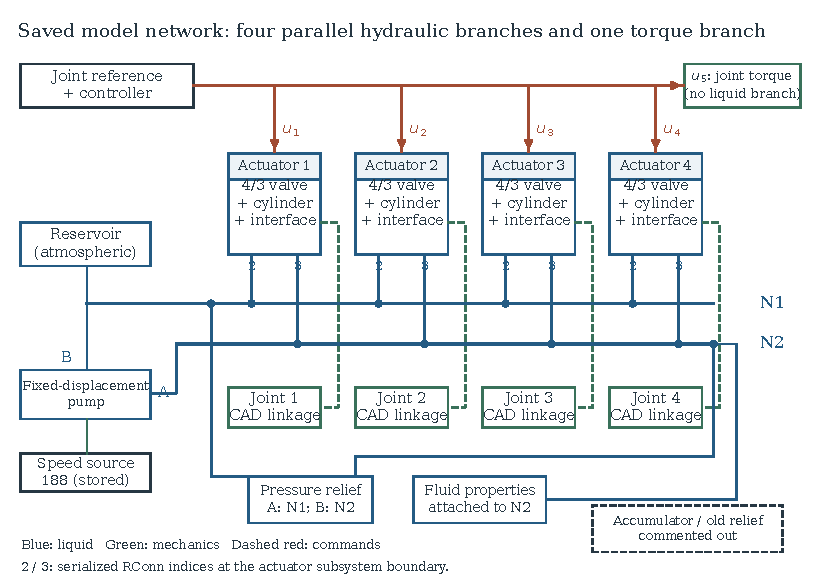
\includegraphics[width=\textwidth]{figures/hydraulic-network.pdf}
\caption{Complete connection-group reconstruction of the saved model. N1 and N2 name the reservoir-connected and sensor/fluid-connected rails, respectively. Serialized connector indices are retained at subsystem boundaries; they require a compiled port/sign check before being interpreted as a validated operating circuit. Blue lines show liquid connectivity, green denotes mechanical coupling, and dashed red denotes commands. The four hydraulic modules share both rails; the fifth command bypasses the liquid network. Commented components have no active branch. This diagram represents connectivity, not measured flow direction.}
\label{fig:network}
\end{figure*}

\begin{table*}[t]
\caption{Documented Design Versus Activation in the Saved Editable Model}
\label{tab:state}
\centering\small
\begin{tabular}{p{.24\textwidth}p{.26\textwidth}p{.42\textwidth}}
\hline
Component/effect & Saved state & Interpretation\\\hline
Four valve/cylinder/friction branches & Active replacement blocks & Use these parameters rather than commented predecessors.\\
Gas-charged accumulator & Commented out & The saved configuration does not provide accumulator buffering.\\
Older relief and fluid-properties blocks & Commented out & The active relief and \textnormal{Hydraulic Fluid} block define the retained configuration.\\
Built-in cylinder friction/leakage & Disabled on active cylinders & External friction remains active; internal leakage is not enabled there.\\
Explicit pipe/hose elements & Not present in the main circuit inventory & A separate distributed line-compliance or hose-wave model is not established by this network.\\
Fifth axis & Direct torque-command conversion & Five commands do not imply five valve-controlled cylinders.\\
End-effector error functions at root & Commented out & Enable a consistent logging/evaluation path before recomputing tracking errors.\\\hline
\end{tabular}
\end{table*}

The Connection Port blocks inside each actuator are named C$i$, R$i$, P, and T, with stored port numbers 1--4. Because left/right connector indices, flexible port placement, and rotated library blocks are distinct representations, the association of the named P/T ports to each top-level rail must be confirmed with the loaded model~\cite{connectionport}. The saved rail groups and the original presentation are not sufficient to certify pump rotation, relief opening direction, or pressure-boundary placement. A reproducible run should record compiled port handles and a small open-loop pressure/flow test before closing the position loop.

\subsection{Supply Parameters and Unit Consistency}
The presentation gives a nominal flow scale of 40~L/min and a pressure range of 280--360~bar. These are design-context values, not a complete parameterization of the saved pump. Table~\ref{tab:supply} lists the active record. In particular, the pump displacement field is stored as 25 with unit m$^3$/rad. Combining that literal field with an interpreted 188~rad/s speed would produce an implausible geometric-flow scale; it must not be relabeled as 25~cm$^3$/rev without checking and correcting the model. The report records this discrepancy rather than claiming the stored pump realizes 40~L/min.

\begin{table}[t]
\caption{Selected Active Supply and Fluid Parameters}
\label{tab:supply}
\centering\small
\begin{tabular}{@{}p{.44\columnwidth}p{.48\columnwidth}@{}}
\hline
Stored quantity & Value and unit\\\hline
Pump displacement & 25 m$^3$/rad (saved field)\\
Pump speed source & 188; source unit stored as 1\\
Relief differential set pressure & 27.579 MPa\\
Relief pressure range & 2.759 MPa\\
Liquid density at atmosphere & 845 kg/m$^3$\\
Liquid bulk modulus & 1.5 GPa\\
Kinematic viscosity & 52.6297 cSt\\
Stored entrained-air fraction & 0.004\\
Reservoir pressure specification & Atmospheric\\\hline
\end{tabular}
\end{table}

The active fluid-properties block stores a constant liquid bulk-modulus option and the air-related parameters. A stored field is not proof that every option-dependent effect is active. A new bulk-modulus sweep must identify the particular active block field being varied, preserve all other settings, and save the evaluated parameter set. Likewise, the nominal 34~MPa supply value in a helper file is not the same quantity as the active relief differential setpoint of 27.579~MPa.

\subsection{Valve Routing and Command Conversion}
Figure~\ref{fig:valve} expands the valve symbol. The active directional-valve configuration lists P--A and B--T for positive spool displacement, all nominal paths closed in neutral, and P--B and A--T for negative displacement~\cite{valve}. These are valve-relative paths; extension direction still depends on the cylinder orientation, port connection, and linkage geometry. A nominally closed center also retains the finite stored leakage opening and does not establish exact load holding.

\begin{figure*}[t]
\centering
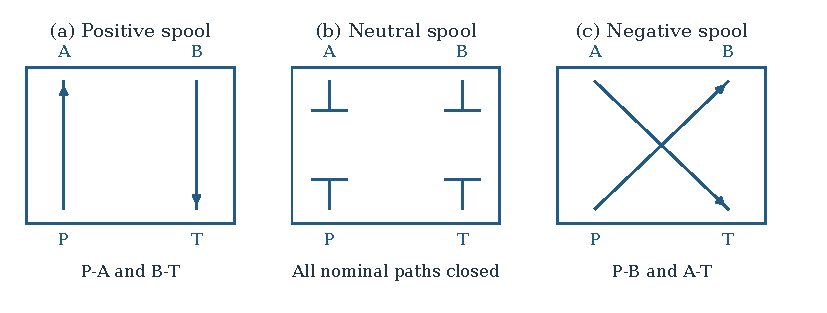
\includegraphics[width=\textwidth]{figures/valve-routing.pdf}
\caption{Metering paths selected by the active 4-way, 3-position valve configuration. Positive spool displacement connects P to A and B to T; negative displacement reverses the chamber connections. At neutral the nominal paths are closed, with a finite leakage-area floor in the block parameterization. Arrows illustrate valve-relative routing under the usual pressure ordering, not a verified flow direction in the saved network.}
\label{fig:valve}
\end{figure*}

The four active valves share a maximum orifice-area field of 500~mm$^2$, leakage-area field of $10^{-12}$~m$^2$, discharge coefficient 0.7, and critical Reynolds number 12. The common spool-travel expression is approximately 0.005~m; several path-specific fields are also retained. Their interpretation depends on the active valve-area parameterization, so inactive alternative fields should not be mixed into one metering law.

Each command passes through a Simulink--PS Converter configured with unit m. Its stored mode is \textnormal{provide}, with user-provided derivative value zero. Although an input-filter time-constant field of 0.005~s exists, this field alone does not demonstrate an enabled first-order spool filter. The controller clips dimensionless-looking numeric commands near unity, whereas the converter declares displacement in metres. The command-to-spool scale therefore needs an explicit unit check against the roughly 5~mm valve travel. Treating the separate legacy custom valve's 0.07~s filter as the active valve dynamics would describe a different implementation.

\subsection{Instrumentation and Data Paths}
Pressure taps on both cylinder chambers connect to pressure-sensor subsystems and PS--Simulink converters. Extension sensing comes from the prismatic position signal; force sensing branches from the interface force signal. Arm revolute joints supply position and velocity. The plant groups these signals into vectors, with stored Unit Delay blocks in the signal-routing subsystem. These discrete delays and the controller's integration interval belong to the measurement/control path, not to the continuous hydraulic chamber equations.

Reference Signal Editor blocks load joint position, velocity, acceleration, and end-effector datasets. The controller uses position and velocity references and measured joint motion; pressure ports exist on the controller function but are unused by its current equations. Supply pressure, chamber pressures, and cylinder strokes are therefore available for diagnostics without constituting pressure feedback control. The root end-effector error functions are commented out in the saved model, so their mere presence does not guarantee an \textnormal{e\_norm} log in a new run.

\subsection{Assembly and Initialization Procedure}
To rebuild the network, first establish one reservoir boundary and the selected fluid-properties and Solver Configuration blocks. Connect the pump shaft, mechanical reference, and speed source; then confirm pump port orientation and the pressure-relief path using pressure and flow signs. Connect one valve/cylinder branch and verify that a small positive and negative spool displacement produce the intended extension and retraction. Only then duplicate the branch for the remaining cylinders and connect the common rails.

Before simulation, reconcile the cylinder's zero-displacement definition with the CAD reference length, evaluate the workspace-dependent offset, and choose compatible chamber pressures and multibody state targets. Enable only the intended friction, leakage, cushioning, and hard-stop contributions. Next, check the command-to-spool conversion, actuator signs, sensor units, and sample times. Close the controller loop after these tests, retain the complete startup transient, and log reference, response, chamber pressures, strokes, valve commands, and tracking error on declared timestamps. This construction procedure explains how to obtain a testable model; it does not substitute for a successfully executed validation run.
